\section{Figure Sample}

\begin{figure}[H]
	\centering
	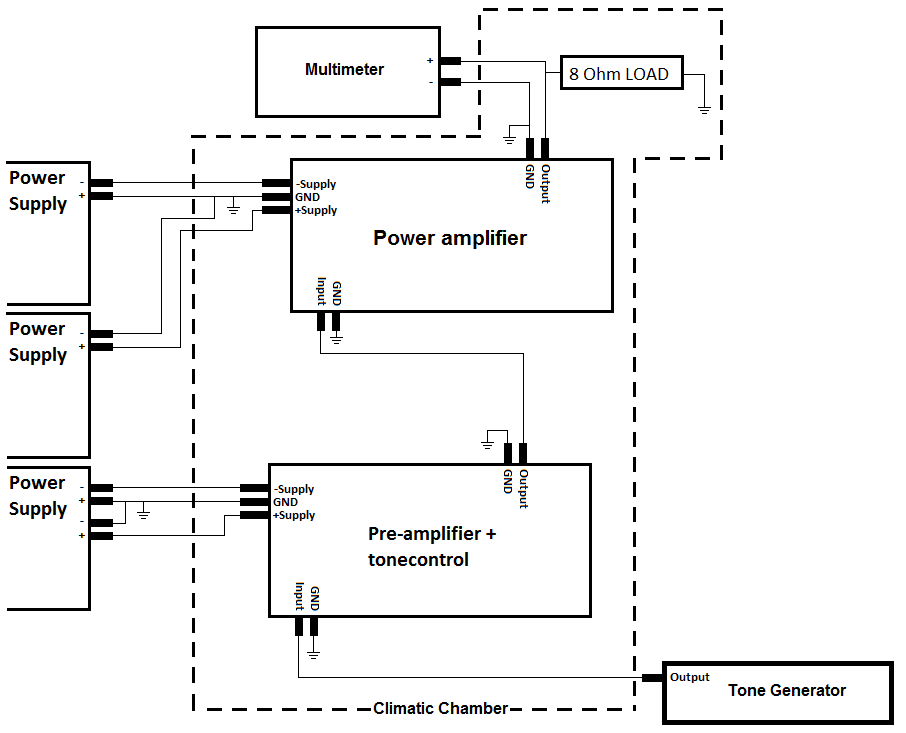
\includegraphics[scale=.6]{figures/filename}
	\caption{CAPTION\fxnote{Remember source}}
	\label{LABEL}
	\flushleft
	\textit{SOURCE}
\end{figure}

%--------- NOTES ------------------------------------------------------
%Fxnotes wont compile properly inside the figure, only in the caption.
%Filetype ([...]{figures/filename.jpg}) can be specified but isn't needed.

\figref{LABEL} \Figref{LABEL}

%Do not use \vspace{length} or \hspace{length} or \noindent etc unless exceedingly necessary - LaTeX is a markup language, let it do its job.
\vspace{.5cm}
\noindent
%--------- BIBLIOGRAPHY REF EKSAMPLE -----------------------------------
This reference only represents this line since it is before the punctuation mark\cite{YDing}. This next reference however represents the entire section. That is all of the preceding sentences in the entire section. This is due to the fact that it is now after the punctuation mark in the end of the section (this is not used in the middle of a section!).\cite{YDing}
%>>>>>>>>>>>>>>>PLEASE ALSO READ THE NOTE IN bibliography/bibliography.bib<<<<<<<<<<<<<<<<<<
\pagebreak